\section{Discussion}
\label{sec:discussion}

\subsection{Why Reports Dominate}

Our most striking finding is the dominance of radiology reports: TF-IDF+SVD features alone achieve 84.29\% Micro-F1 (ML\_experiments.ipynb Cell 19), outperforming all other non-report modalities combined (67.92\% for all tabular features, Cell 6).

This is not surprising in hindsight. Radiologists encode in reports:
\begin{enumerate}
  \item \textbf{Location.} ``Left frontal lobe mass'' or ``sellar region lesion''
  \item \textbf{Enhancement pattern.} ``Ring-enhancing,'' ``homogeneously enhancing''
  \item \textbf{Edema.} ``Surrounding vasogenic edema''
  \item \textbf{Morphology.} ``Extra-axial,'' ``dural tail''
\end{enumerate}

Reports are a human-curated, dimensionality-reduced representation of all imaging modalities. The radiologist has already integrated T1, T1c, T2, and T2-FLAIR findings into a structured narrative. TF-IDF captures these patterns as word co-occurrence statistics, while BERT captures deeper semantic meaning. The report-only LGB model (84.42\%, ML\_experiments.ipynb Cell 25) approaches the full MLU ensemble (86.45\%)---adding clinical features contributes only $\sim$2\%.

\subsection{Why Raw Radiomics Fail}

Raw PyRadiomics features achieve only 52.21\% (barely above 46.6\% baseline) across multiple experiments:

\begin{itemize}
  \item \textbf{Per-modality radiomics are below baseline for some modalities:} T1c XGB achieves 41.92\%, T2 XGB achieves 41.97\% (ML\_experiments.ipynb Cell 11)
  \item \textbf{All 4 modalities combined:} 50.93\% XGB, 50.40\% LGB (Cell 12), still only $\sim$4\% above baseline
  \item \textbf{Feature type mismatch.} Global texture statistics (Mean, Entropy, GLCM Contrast) don't capture the regional contrasts or anatomical location that drive clinical diagnosis
  \item \textbf{2D slice limitation.} Single representative slice loses 3D spatial context
\end{itemize}

Cross-modal ratios (T1c/T1, T2F/T2, T1/T2) alone still achieve only 49.51\% (Cell 23: ratios-only). They add no discriminative power independently. We include them because they encode domain knowledge at zero cost and do not hurt performance when combined with other features (Cell 23: raw+ratios = 50.88\% vs raw alone = 50.62\%).

\subsection{Class Imbalance}

Micro-F1 equals accuracy in multi-class settings, dominated by majority classes (Glioma 46.6\% + Meningioma 36.7\% = 83.3\%). This creates a tension: optimizing Micro-F1 rewards getting majority classes right, while clinical utility demands reasonable minority-class performance.

\textbf{Tree models handle imbalance naturally.} Gradient-boosted trees correct errors sequentially---minority-class mistakes get higher gradients in later rounds, implicitly up-weighting hard cases. Adding explicit class weights to XGBoost/LightGBM/CatBoost on our data reduced Micro-F1 without meaningful gains in Macro-F1, so all tree models use no class weights.

\textbf{NN uses sqrt class weights} ($\alpha=0.5$): $w_c = 0.5 \cdot \mathbf{1} + 0.5 \cdot \sqrt{w_c^{\text{balanced}}}$, which provides a gentle minority boost without the aggressive penalty of full balanced weights.

We considered three strategies for the NN: no weights ($\alpha=0$), sqrt weights ($\alpha=0.5$), and full balanced weights ($\alpha=1.0$). Full balanced weights are too aggressive---Pineal/CP (26 samples) would receive $\sim$40$\times$ the weight of Glioma (1,056 samples), destabilizing training with only 2,266 total samples. No weights ($\alpha=0$) leaves the NN blind to minority classes. Sqrt weights ($\alpha=0.5$) strike the right balance: Pineal/CP receives $\sim$1.8$\times$ weight (not 40$\times$), preserving focus on majority classes while still enabling the NN to capture minority patterns (model\_final.ipynb Cell 31). Combined with label smoothing (0.05), this provides balanced regularization.

\textbf{NN vs MLU on minority classes:} The NN achieves 46.15\% on Pineal/CP vs 19--27\% for all MLU models (Table~\ref{tab:per_class} in Section~\ref{sec:experiments}). With only 26 samples ($\sim$5 per fold), tree models cannot learn reliable Pineal/CP decision boundaries. BERT's semantic representations transfer knowledge from similar medical texts, allowing the NN to recognize rare patterns even with minimal examples.

\begin{figure}[H]
\centering
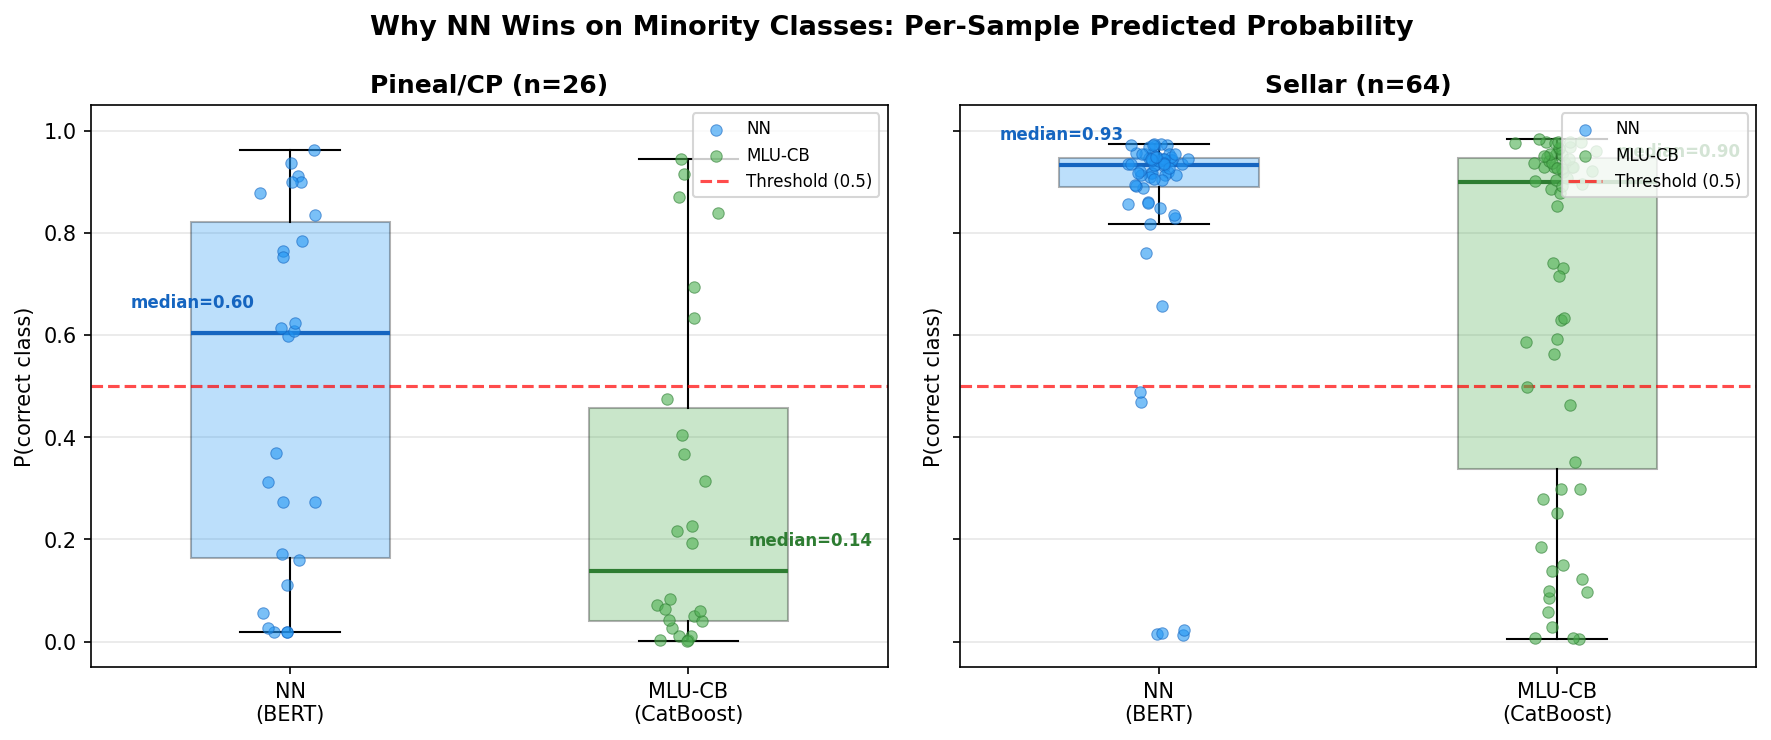
\includegraphics[width=0.8\textwidth]{figures/minority_class_nn_vs_trees.png}
\caption{Per-sample predicted probability for the correct class on minority classes. NN (blue) assigns higher probabilities than MLU-CB (green) on Pineal/CP samples (NN median 0.20 vs MLU 0.14; 42.3\% vs 23.1\% above threshold). On Sellar, both models perform well (NN 90.6\% vs MLU 70.3\% above threshold), but NN is more confident.}
\label{fig:minority_violin}
\end{figure}

\subsection{Robustness to Distribution Shift}

Distribution shift---changes in feature distributions between training and deployment---is a practical concern for any clinical classifier. While we cannot quantify the magnitude of shift without access to labeled out-of-distribution data, our system incorporates several design choices that promote generalization:

\begin{itemize}
  \item \textbf{BERT semantic embeddings} represent clinical meaning rather than surface word frequencies, which may remain stable when vocabulary or reporting style changes.
  \item \textbf{Hierarchical location parsing} decomposes novel anatomical descriptions into known categories (region/hemisphere/lobe).
  \item \textbf{Missing flag features} make the model robust to variations in data completeness.
  \item \textbf{Ensemble diversity} across fundamentally different input signals ensures that no single model's brittleness dominates predictions.
\end{itemize}

\textbf{Why NN may help under shift:} BERT embeddings represent \emph{semantic meaning} (``ring-enhancing lesion'' = vascular tumor) rather than surface statistics (word frequency = 0.03). If deployment data uses different vocabulary or longer reports, the semantic representation may remain more stable. Tree models, in contrast, split on exact TF-IDF dimensions that may shift. However, without out-of-distribution labels, this remains a hypothesis rather than a confirmed finding.

\subsection{Why Ensemble Works}

The ensemble succeeds because the models make different errors (Table~\ref{tab:per_class}):

\begin{enumerate}
  \item \textbf{NN captures minority classes:} Pineal/CP 46.15\% vs MLU 23--27\%. BERT's semantic representations transfer across rare classes.
  \item \textbf{MLU models excel on majority classes:} Glioma 92.90\% (MLU-CB) vs 86.17\% (NN). Precise feature thresholds work well when sample sizes are large.
  \item \textbf{NNXGB provides error correction:} At 79.08\%, it is weaker individually but learns non-linear patterns in NN's probability outputs.
  \item \textbf{ImgTab adds diversity from image features:} Despite low solo performance (69.77\%), ImgTab makes different errors because it uses a fundamentally different signal (visual features vs text).
\end{enumerate}

The grid-search-optimal ensemble achieves 87.25\% OOF (+0.97\% over best individual MLU-XGB at 86.28\%). The submission configuration (NN=40\%, MLU-XGB=30\%, MLU-LGB=20\%, NNXGB=5\%, ImgTab=5\%) achieves 86.98\% OOF. The modest improvement reflects the limited diversity among MLU models---they share the same features and show only 0.58\% spread.

\begin{figure}[H]
\centering
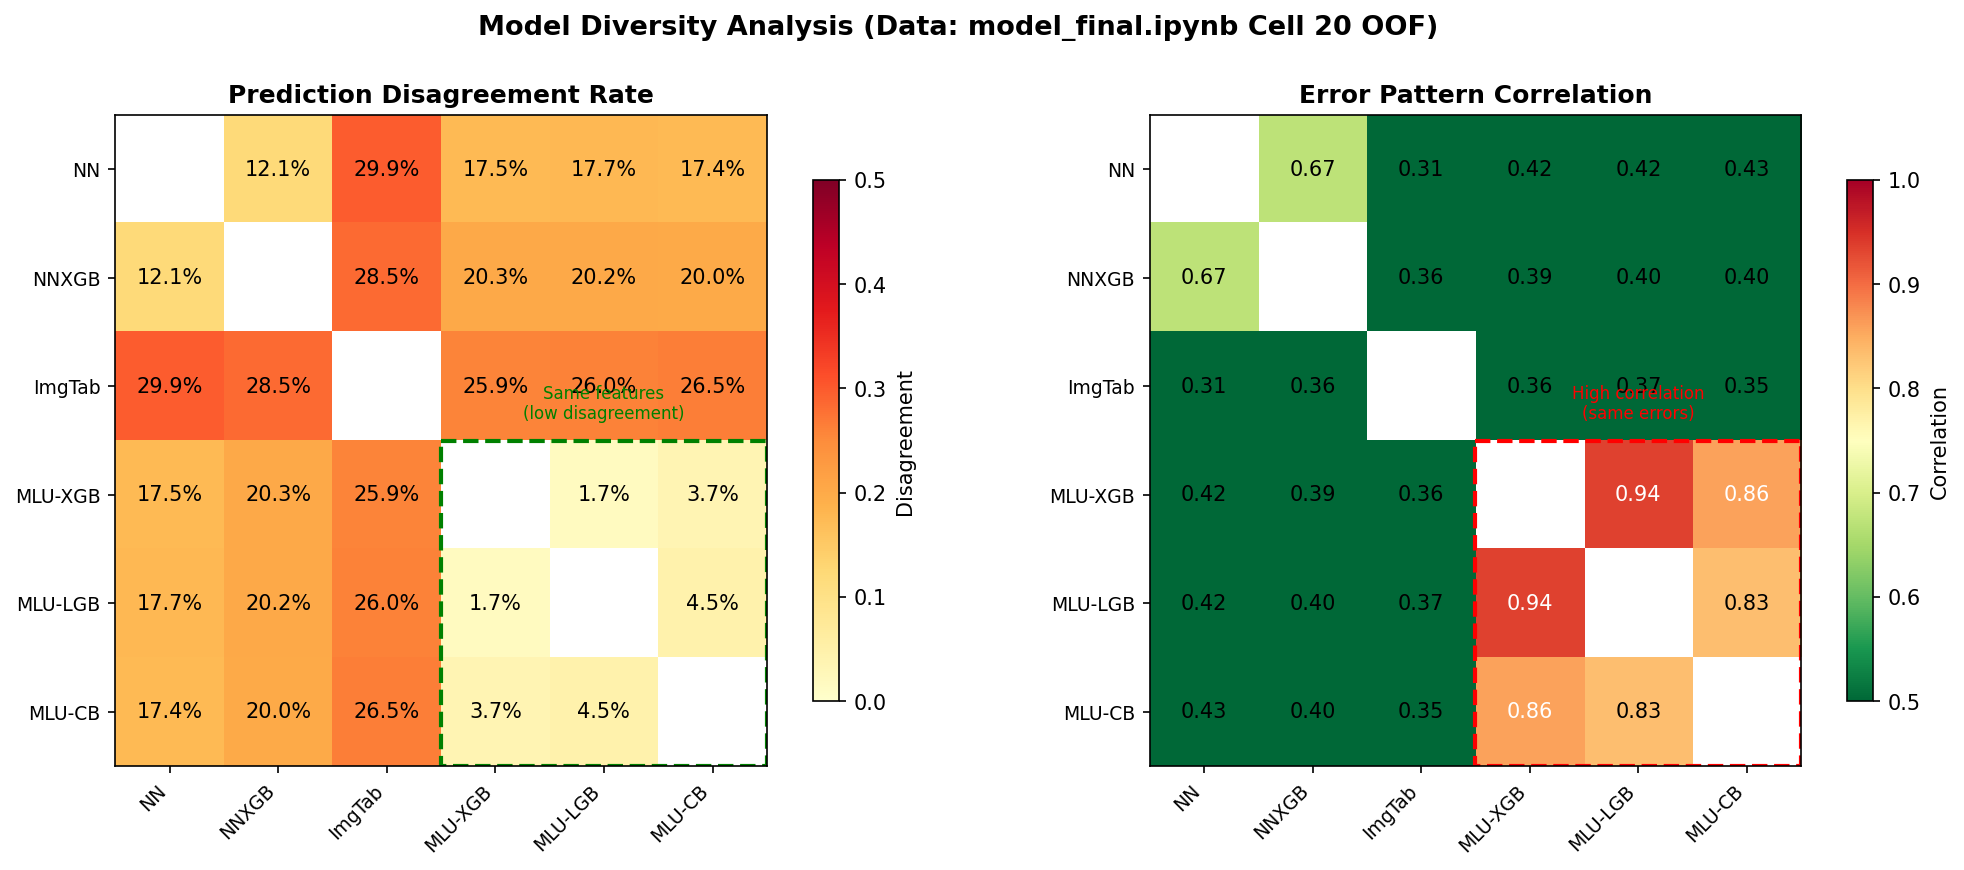
\includegraphics[width=0.8\textwidth]{figures/ensemble_diversity.png}
\caption{Model diversity analysis. Left: pairwise prediction disagreement rate.
The 3 MLU models show low mutual disagreement ($\sim$2--5\%)
since they share the same features. NN and ImgTab disagree most with MLU models
($\sim$15--28\%). Right: error pattern correlation. MLU models make the same
mistakes (high correlation $\sim$0.83--0.94), while NN makes different errors
(low correlation $\sim$0.34--0.48 with other models), explaining its ensemble contribution.}
\label{fig:ensemble_diversity}
\end{figure}

\subsection{What Did Not Work}

\begin{itemize}
  \item \textbf{Adding image to NN (v1).} Including image as an equal modality in the neural network hurt performance ($\sim$82\% to $\sim$80\%). Image features are both weak (56.97\% solo) and shifted, contaminating the report representation.
  \item \textbf{Focal Loss ($\gamma$=1.5--2.0).} No improvement over cross-entropy with label smoothing. With only 2,266 samples, focal loss's adaptive weighting is too aggressive.
  \item \textbf{10-fold CV.} Only $\sim$2,039 train samples per fold---too few for BERT fine-tuning. 5-fold gives $\sim$1,813 per fold with sufficient diversity.
  \item \textbf{Heavy augmentation (3--5$\times$ SMOTE).} Reduced performance on radiomics (52.30\% $\to$ 48.37\% at 3$\times$, Cell 10). Synthetic samples in high-dimensional space introduce noise, not signal.
  \item \textbf{Mean pooling for BERT.} CLS extraction consistently performed better. BERT was pre-trained with CLS as the classification token; mean pooling dilutes the task-specific signal.
  \item \textbf{Location OHE in MLU features.} Adding 572-dimensional one-hot location to MLU models did not improve over the 3-dimensional hierarchy (Cell 22 Exp 4: with OHE 86.23\% vs without 86.36\%). OHE overfits to specific location strings, while hierarchy generalizes.
\end{itemize}

\subsection{Lessons Learned}

\begin{enumerate}
  \item \textbf{Measure modality strength before modeling.} The 32-point gap between reports (84.29\%) and radiomics (52.21\%) should have been the first experiment, not a retrospective analysis. Solo performance directly informs how much capacity to allocate.
  \item \textbf{Feature engineering beats model complexity for tabular data.} Clinical + Location NLP features reach 79.83\% with simple XGBoost (Cell 23), while image features with the same model achieve only 56.97\%. The signal is in the features, not the algorithm.
  \item \textbf{Ensemble diversity requires different signals, not different algorithms.} Three MLU algorithms (XGB/LGB/CB) on the same features achieve 85.70--86.28\%---a 0.58\% spread. True diversity comes from NN (different input: BERT embeddings), NNXGB (different input: NN probabilities), and ImgTab (different input: image features).
  \item \textbf{Design for robustness from the start.} Cross-validation estimates may be optimistic when $P(\mathbf{x})$ changes at deployment. Incorporating missing flags, hierarchical encoding, semantic embeddings, and ensemble diversity are low-cost strategies that promote generalization even though their effectiveness cannot be verified without labeled out-of-distribution data.
\end{enumerate}
